\documentclass[a4paper, oneside]{memoir}
\usepackage[utf8]{inputenc}
\usepackage[T1]{fontenc}
\usepackage{pifont}
\usepackage{amssymb}
\usepackage{fourier}
\usepackage[dvipsnames]{xcolor}
\usepackage{tikz}
\usepackage{pdfpages}
\usepackage[sfdefault]{roboto}
\usepackage{color}

% Styles
\tikzstyle{teamshare} = [below, text width=5.4cm, inner sep = 0.5cm, text=white, align=center]
\tikzstyle{cardtext} = [below, text width=5.9cm, inner sep = 0.25cm, text centered]
\setlrmarginsandblock{0.9cm}{*}{1}
\setulmarginsandblock{1.2cm}{*}{1}
\checkandfixthelayout[nearest]
\pagestyle{empty}

% Define Commands
\newcommand{\condition}[1]{\textbf{#1}}
\newcommand{\character}[1]{\textbf{#1}}
\newdimen\titlespacing
\titlespacing=0.15cm

% Define Seperators
\newcommand{\seperator}[1]{\\ \vspace{\titlespacing} \hrulefill {} \tiny \bfseries #1 \normalfont \normalsize \hrulefill \\ \vspace{\titlespacing}}
\newcommand{\seperatoraction}{\seperator{POWER}}
\newcommand{\seperatordescription}{\seperator{DESCRIPTION}}
\newcommand{\seperatorcondition}{\seperator{CONDITION}}
\newcommand{\seperatorwin}{\seperator{HOW TO WIN}}
\newcommand{\redwinsection}{
	\seperatorwin
	You win if \character{Harry Potter} does not gain the \condition{dead} condition due to \character{Voldemort}.
}
\newcommand{\greenwinsection}{
	\seperatorwin
	\small You win if \character{Harry Potter} gains the \condition{dead} condition due to the \character{Voldemort}.
}
\newcommand{\titlefrom}[1]{\\ \tiny > from #1 <\normalsize}

% Begin Document
\begin{document}
\noindent 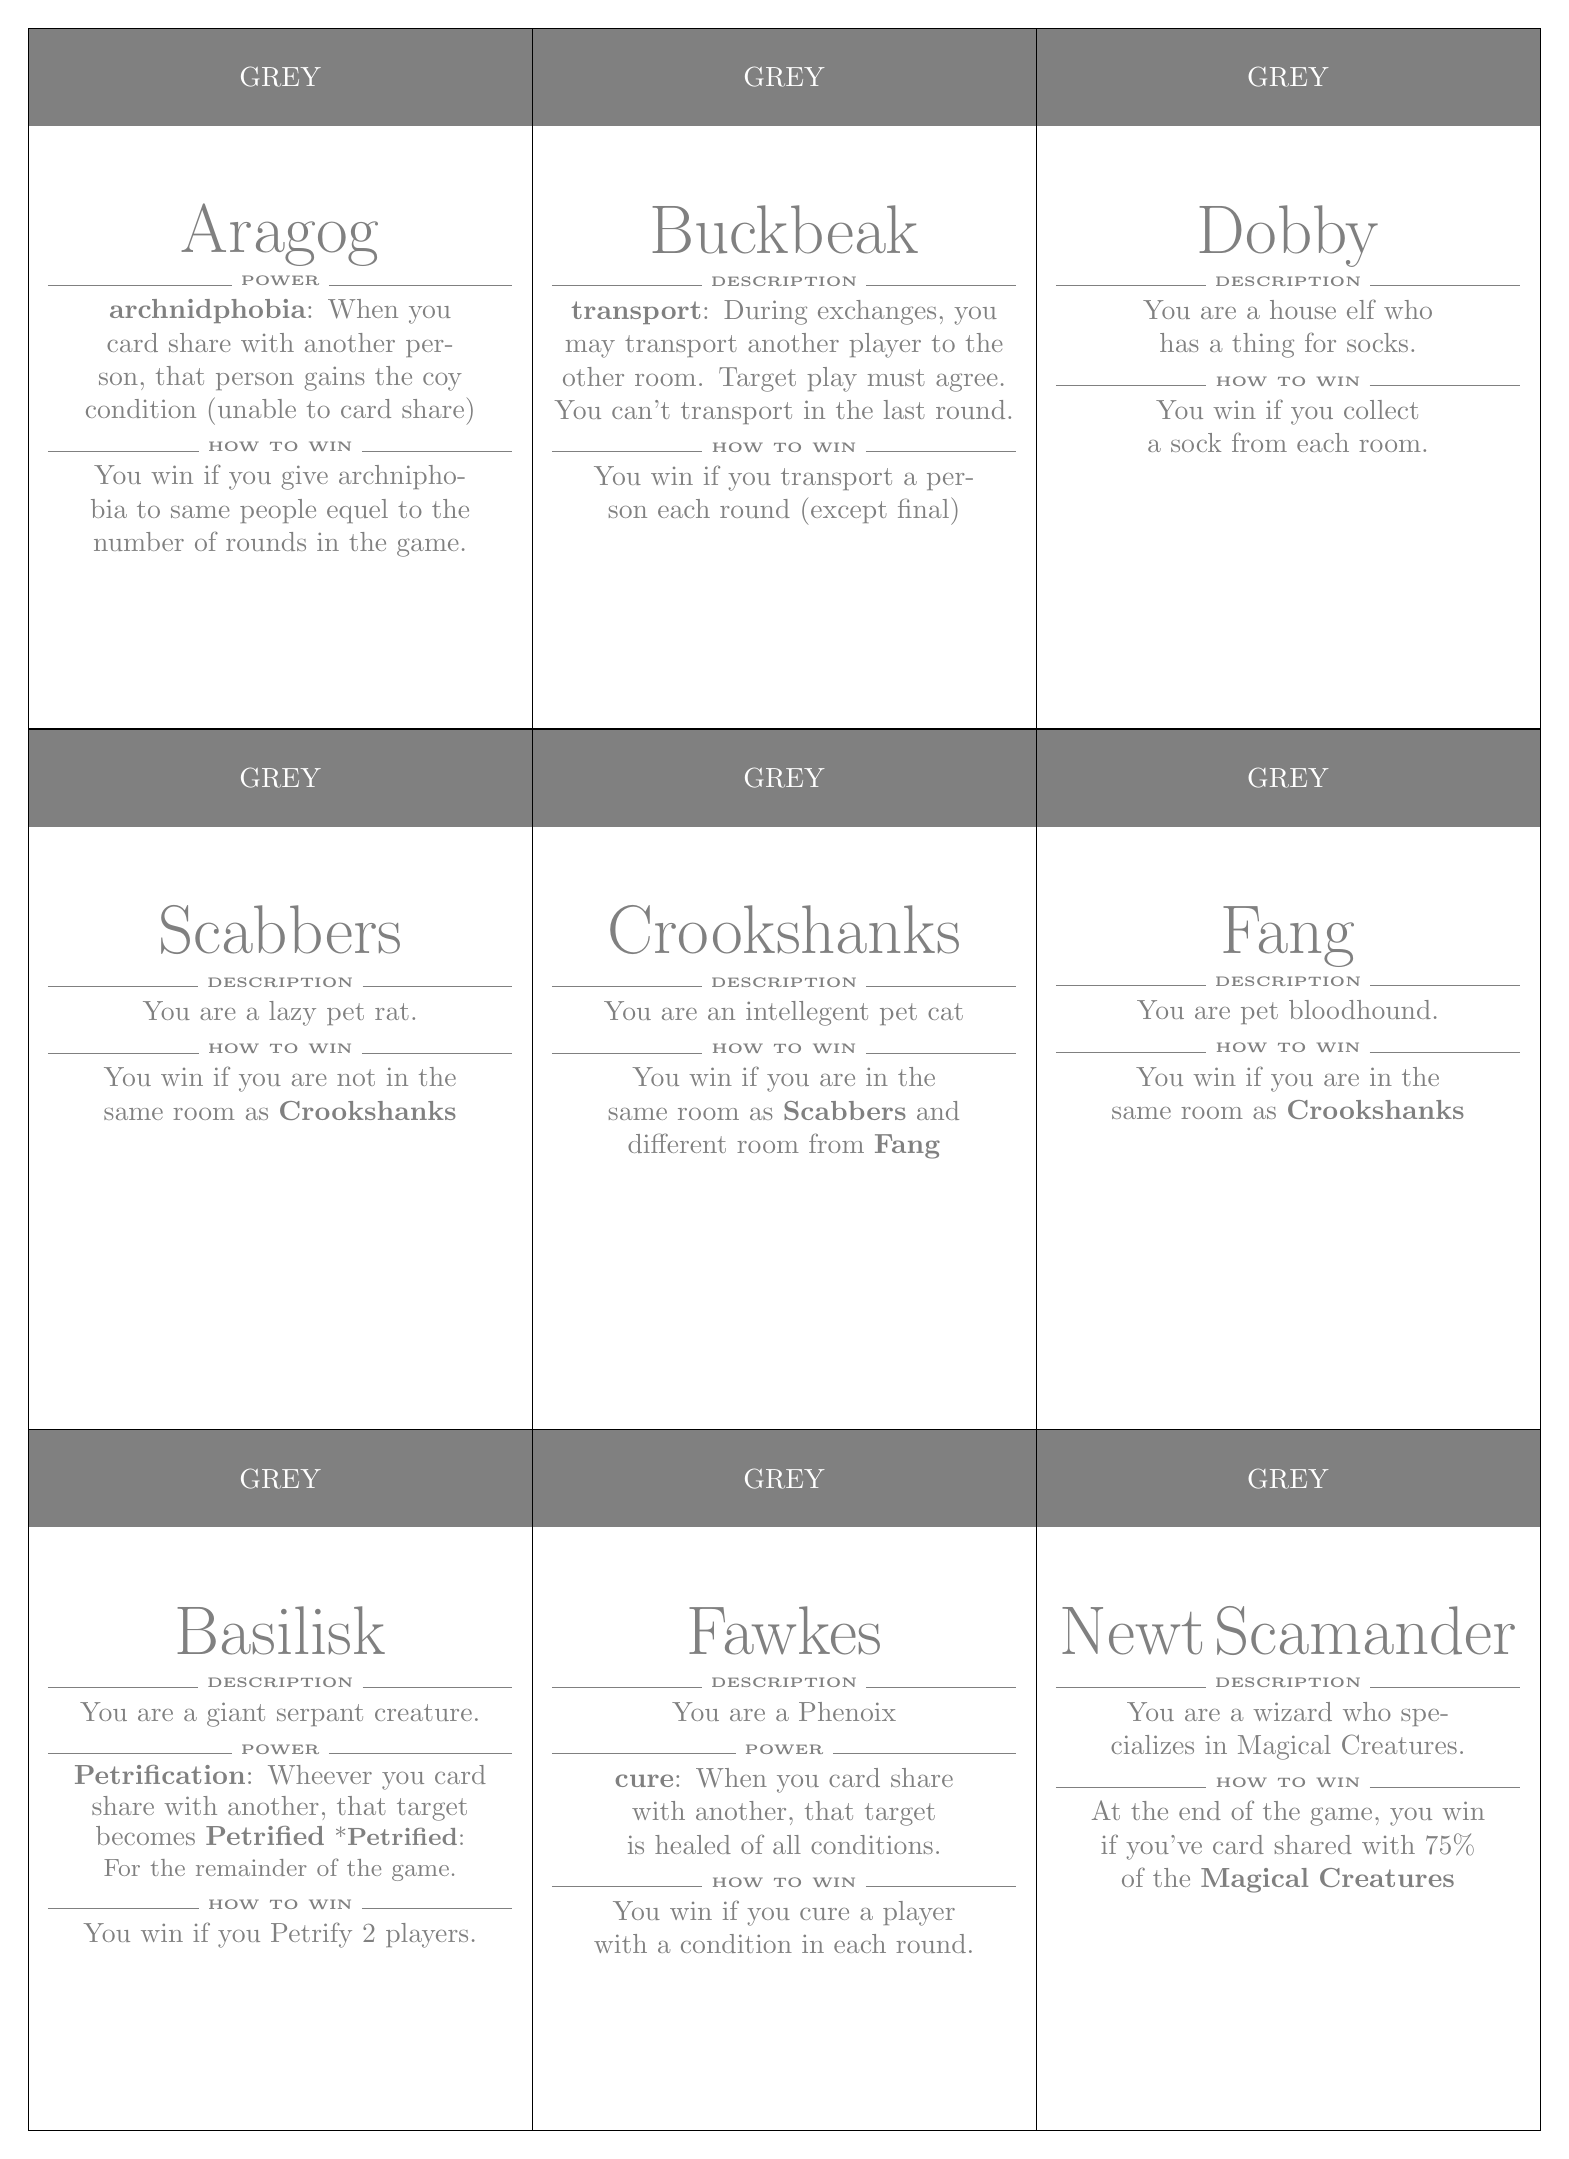
\begin{tikzpicture}[outer sep=0]

	% ARAGOG
	\node[teamshare, fill=gray] (1) at (3.2,26.7) {\HUGE GREY};
	\node[cardtext, text=gray] at (3.2,24.7) {
		{\Huge Aragog}
		\seperatoraction
		\condition{archnidphobia}: When you card share with another person, that person gains the coy condition (unable to card share)
		\seperatorwin
		You win if you give archniphobia to same people equel to the number of rounds in the game.
	};
	
	% BUCKBEAK
	\node[teamshare, fill=gray] at (9.6,26.7) {\HUGE GREY};
	\node[cardtext, text=gray] at (9.6,24.7) {
		{\Huge Buckbeak}
		\seperatordescription
		\condition{transport}: During exchanges, you may transport another player to the other room. Target play must agree. You can't transport in the last round.
		\seperatorwin
		You win if you transport a person each round (except final)
	};
	
	% DOBBY (HOUSE ELF)
	\node[teamshare, fill=gray] at (16,26.7) {\HUGE GREY};
	\node[cardtext, text=gray] at (16,24.7) {
		{\Huge Dobby}
		\seperatordescription
		You are a house elf who has a thing for socks.
		\seperatorwin
		You win if you collect a sock from each room.
	};
	
	% SCABBERS THE RAT
	\node[teamshare, fill=gray] at (3.2,17.8) {\HUGE GREY};
	\node[cardtext, text=gray] at (3.2,15.8) {
		{\Huge Scabbers}
		\seperatordescription
		You are a lazy pet rat.
		\seperatorwin
		You win if you are not in the same room as \character{Crookshanks}
	};
	
	% CROOCKSHANKS THE CAT
	\node[teamshare, fill=gray] at (9.6,17.8) {\HUGE GREY};
	\node[cardtext, text=gray] at (9.6,15.8) {
		{\Huge Crookshanks}
		\seperatordescription
		You are an intellegent pet cat
		\seperatorwin
		You win if you are in the same room as \character{Scabbers} and different room from \character{Fang}
	};
	
	% FANG THE BLOODHOUND
	\node[teamshare, fill=gray] at (16,17.8) {\HUGE GREY};
	\node[cardtext, text=gray] at (16,15.8) {
		{\Huge Fang}
		\seperatordescription
		You are pet bloodhound.
		\seperatorwin
		You win if you are in the same room as \character{Crookshanks}
	};
	
	% BASILISK
	\node[teamshare, fill=gray] at (3.2,8.9) {\HUGE GREY};
	\node[cardtext, text=gray] at (3.2,6.9) {
		{\Huge Basilisk}
		\seperatordescription
		You are a giant serpant creature.
		\seperatoraction
		\condition{Petrification}: Wheever you card share with another, that target becomes \condition{Petrified}
		\small *\condition{Petrified}: For the remainder of the game.
		\seperatorwin
		You win if you Petrify 2 players.
	};
	
	% FAWKES THE PHENOIX}
	\node[teamshare, fill=gray] at (9.6,8.9) {\HUGE GREY};
	\node[cardtext, text=gray] at (9.6,6.9) {
		{\Huge Fawkes}
		\seperatordescription
		You are a Phenoix
		\seperatoraction
		\condition{cure}: When you card share with another, that target is healed of all conditions.
		\seperatorwin
		You win if you cure a player with a condition in each round.
	};
	
	% NEWT SCAMANDER
	\node[teamshare, fill=gray] at (16,8.9) {\HUGE GREY};
	\node[cardtext, text=gray] at (16,6.9) {
		{\Huge Newt Scamander}
		\seperatordescription
		You are a wizard who specializes in Magical Creatures.
		\seperatorwin
		At the end of the game, you win if you've card shared with 75\% of the \character{Magical Creatures} 
	};
	
	\draw (0,0) -- (19.2,0);
	\draw (0,8.9) -- (19.2,8.9);
	\draw (0,17.8) -- (19.2,17.8);
	\draw (0,26.7) -- (19.2,26.7);
	\draw (0,0) -- (0,26.7);
	\draw (6.4,0) -- (6.4,26.7);
	\draw (12.8,0) -- (12.8,26.7);
	\draw (19.2,0) -- (19.2,26.7);

\end{tikzpicture}
\includepdf[pages={1}, angle=0]{cardsbackground.pdf}
\pagebreak

\noindent 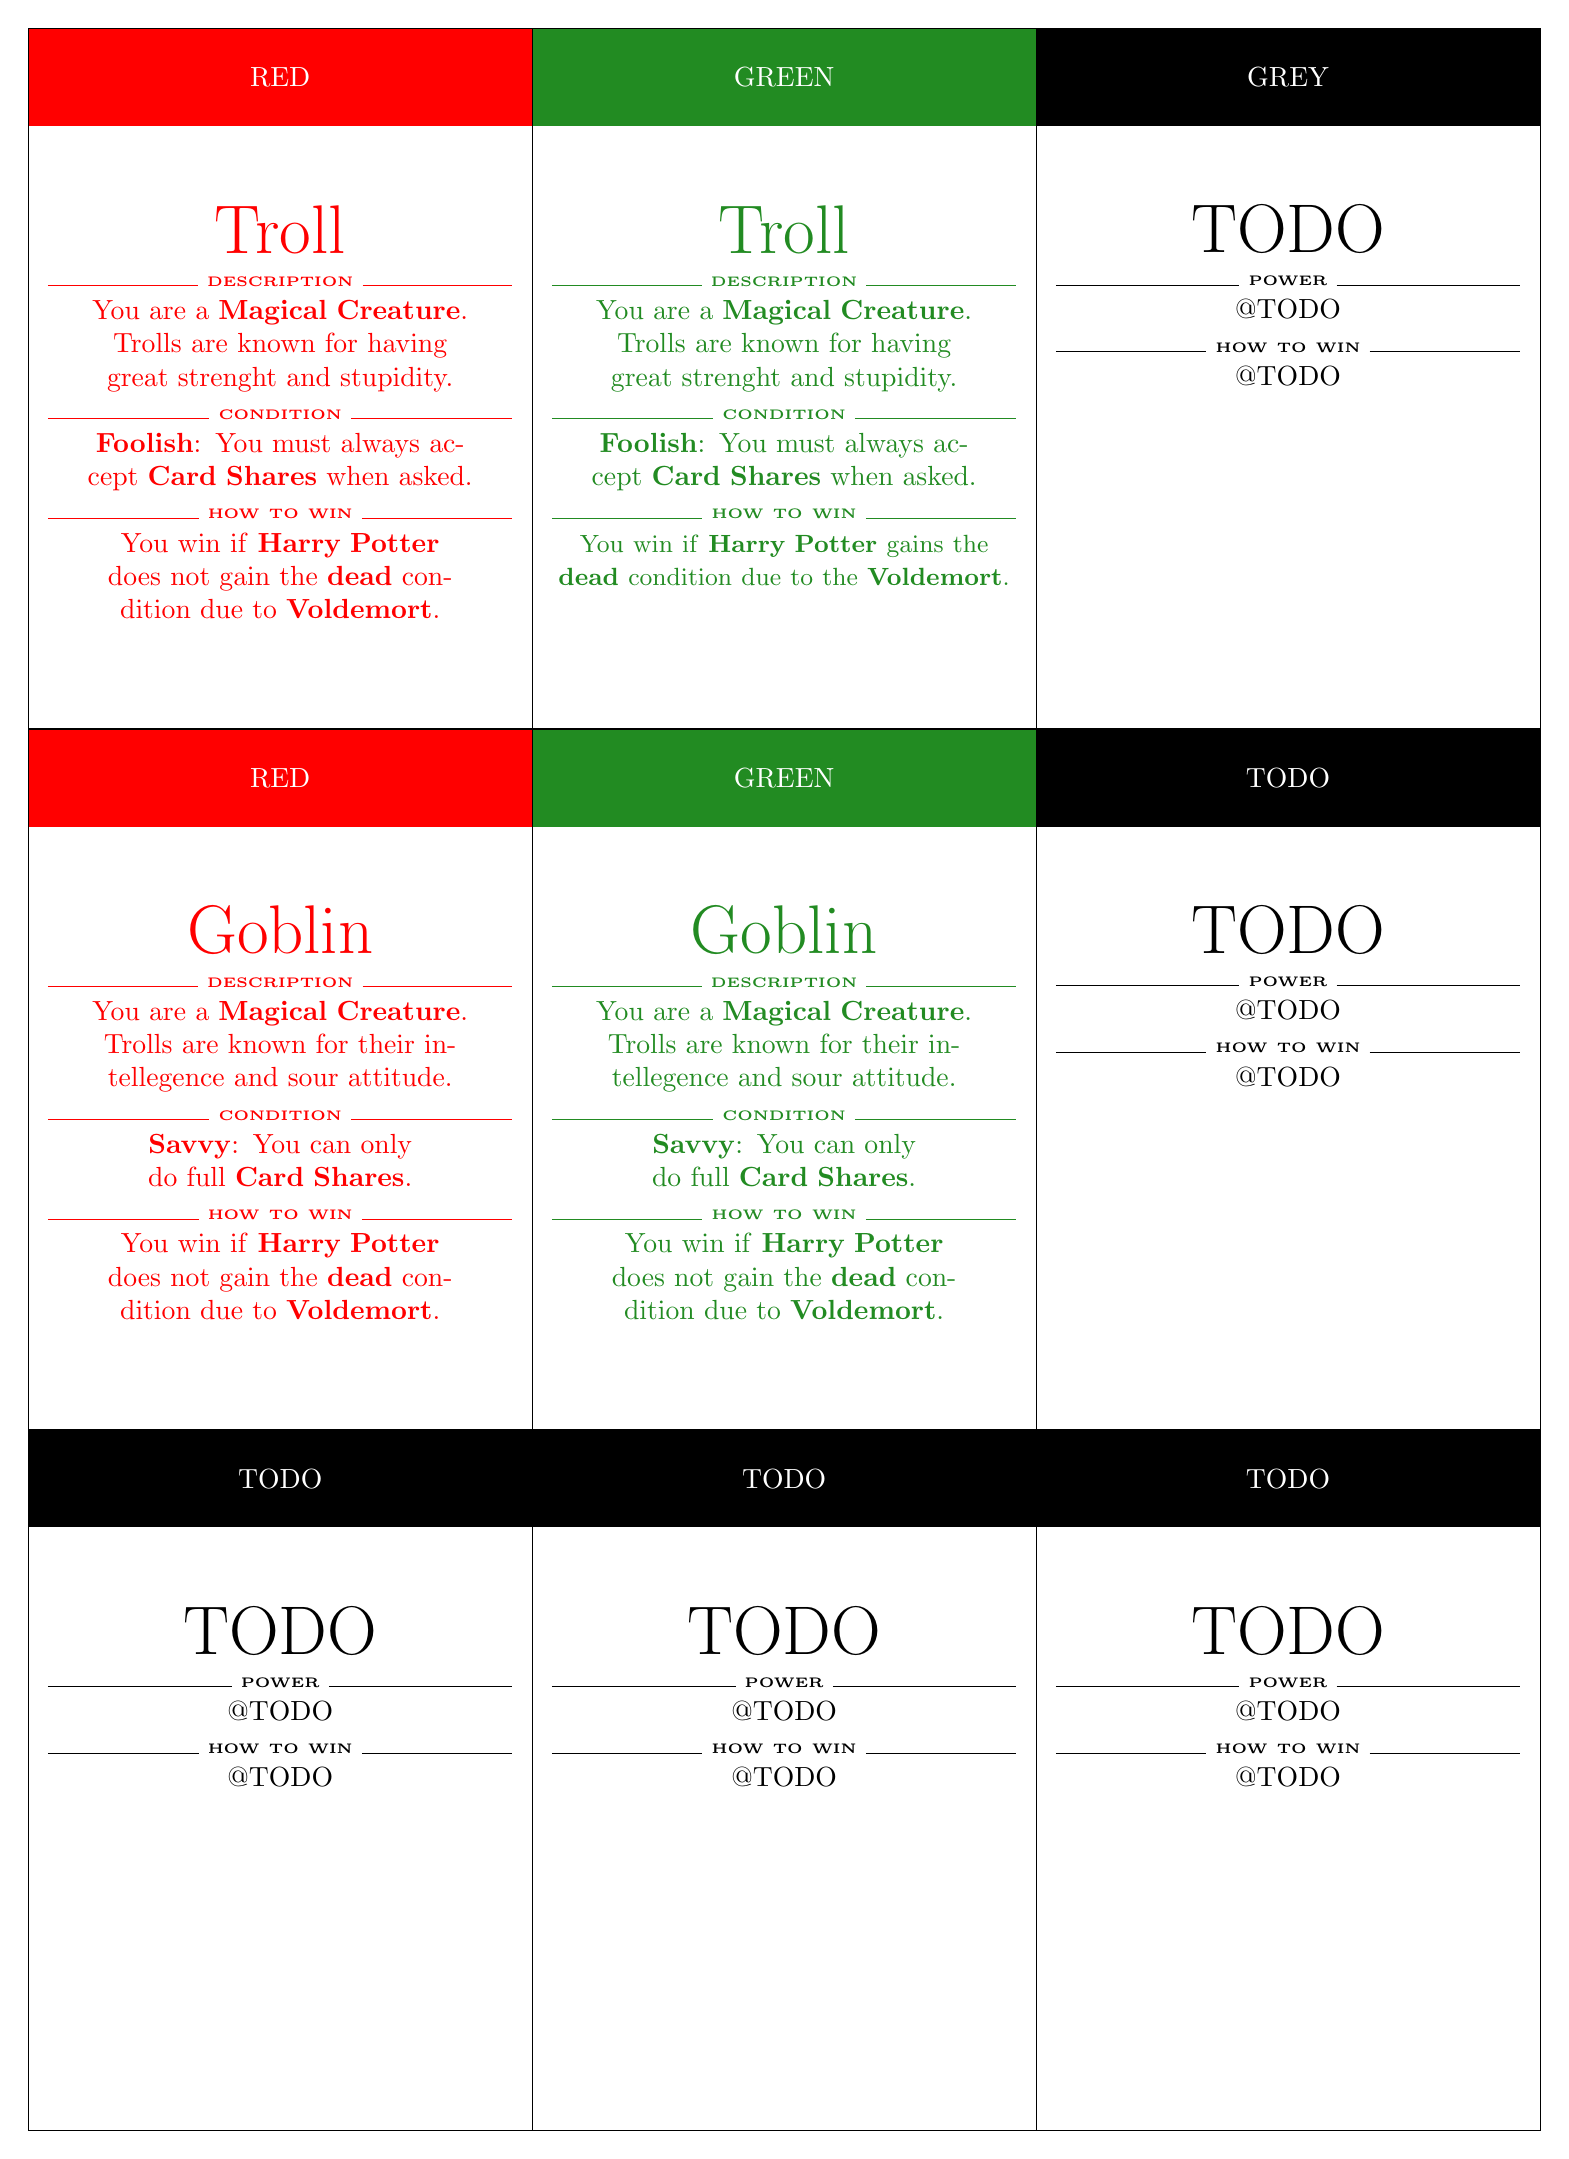
\begin{tikzpicture}[outer sep=0]

	% TROLL (AKA FOOLISH)
	\node[teamshare, fill=red] (1) at (3.2,26.7) {\HUGE RED};
	\node[cardtext, text=red] at (3.2,24.7) {
		{\Huge Troll }
		\seperatordescription
		You are a \condition{Magical Creature}. Trolls are known for having great strenght and stupidity.
		\seperatorcondition
		\condition{Foolish}: You must always accept \condition{Card Shares} when asked.
		\redwinsection
	};
	
	% TROLL (AKA FOOLISH)
	\node[teamshare, fill=ForestGreen] at (9.6,26.7) {\HUGE GREEN};
	\node[cardtext, text=ForestGreen] at (9.6,24.7) {
		{\Huge Troll }
		\seperatordescription
		You are a \condition{Magical Creature}. Trolls are known for having great strenght and stupidity.
		\seperatorcondition
		\condition{Foolish}: You must always accept \condition{Card Shares} when asked.
		\greenwinsection
	};
	
	% TODO
	\node[teamshare, fill=black] at (16,26.7) {\HUGE GREY};
	\node[cardtext, text=black] at (16,24.7) {
		{\Huge TODO}
		\seperatoraction
		@TODO
		\seperatorwin
		@TODO
	};
	
	% GOBLIN (AKA NEGOTIATOR)
	\node[teamshare, fill=red] at (3.2,17.8) {\HUGE RED};
	\node[cardtext, text=red] at (3.2,15.8) {
		{\Huge Goblin}
		\seperatordescription
		You are a \condition{Magical Creature}. Trolls are known for their intellegence and sour attitude.
		\seperatorcondition
		\condition{Savvy}: You can only do full \condition{Card Shares}.
		\redwinsection
	};
	
	% GOBLIN (AKA NEGOTIATOR)
	\node[teamshare, fill=ForestGreen] at (9.6,17.8) {\HUGE GREEN};
	\node[cardtext, text=ForestGreen] at (9.6,15.8) {
		{\Huge Goblin}
		\seperatordescription
		You are a \condition{Magical Creature}. Trolls are known for their intellegence and sour attitude.
		\seperatorcondition
		\condition{Savvy}: You can only do full \condition{Card Shares}.
		\redwinsection
	};
	
	% TODO
	\node[teamshare, fill=black] at (16,17.8) {\HUGE TODO};
	\node[cardtext, text=black] at (16,15.8) {
		{\Huge TODO}
		\seperatoraction
		@TODO
		\seperatorwin
		@TODO
	};
	
	% TODO
	\node[teamshare, fill=black] at (3.2,8.9) {\HUGE TODO};
	\node[cardtext, text=black] at (3.2,6.9) {
		{\Huge TODO}
		\seperatoraction
		@TODO
		\seperatorwin
		@TODO
	};
	
	% TODO
	\node[teamshare, fill=black] at (9.6,8.9) {\HUGE TODO};
	\node[cardtext, text=black] at (9.6,6.9) {
		{\Huge TODO}
		\seperatoraction
		@TODO
		\seperatorwin
		@TODO
	};
	
	% TODO
	\node[teamshare, fill=black] at (16,8.9) {\HUGE TODO};
	\node[cardtext, text=black] at (16,6.9) {
		{\Huge TODO}
		\seperatoraction
		@TODO
		\seperatorwin
		@TODO
	};
	
	\draw (0,0) -- (19.2,0);
	\draw (0,8.9) -- (19.2,8.9);
	\draw (0,17.8) -- (19.2,17.8);
	\draw (0,26.7) -- (19.2,26.7);
	\draw (0,0) -- (0,26.7);
	\draw (6.4,0) -- (6.4,26.7);
	\draw (12.8,0) -- (12.8,26.7);
	\draw (19.2,0) -- (19.2,26.7);

\end{tikzpicture}
\includepdf[pages={1}, angle=0]{cardsbackground.pdf}








\end{document}